\section{Ransac mit Maskierung \dcfirstauthorshort}
\label{sec:evaluation:ransac}

Aus einem Foto mittels \gls{acr:ransac} eine mathematische Approximation einer Fahrbahnmarkierung zu erhalten, war die von uns anfangs angestrebte Herangehensweise. Durch unser Paradigma, eine Weltkarte aufzubauen, ist der Gedanke naheliegend, deren Information zur Verarbeitung eines Bildes zu nutzen. Voraussetzung dafür ist allerdings, dass die Informationen der Karte hinreichend genau sind.

\subsection{Vorteile}
Eine kubische Funktion als mathematisches Modell der gesuchten Linie bietet einige Vorteile:
\begin{itemize}
\item Im Gegensatz zu einer Geraden, einem Kreis oder einer quadratischen Funktion kann das gewählte Polynom dritten Grades zusätzlich dem Verlauf einer S-Kurve (Übergang einer Links- in eine Rechtskurve und umgekehrt) relativ gut folgen. 
%\item Unter der Annahme einer guten Annäherung zur echten Markierung kann im Falle eines unbrauchbaren Fotos durch Extrapolation trotzdem weitergefahren werden. 
\item Unter der Annahme einer guten Annäherung zur echten Markierung kann durch Extrapolation eine wahrscheinliche Vorhersage des Linienverlaufs in einem später aufgenommenen Bild getroffen werden. 
\item Die Stetigkeit der kubischen Funktion verhindert das plötzliche Abknicken des Linienverlaufs, sodass nahezu senkrecht auftreffende Querstraßenmarkierungen nicht als Kurve erkannt werden
\item Durch die Anwendung von \gls{acr:ransac} haben Unterbrechungen oder kleine Störungen keinen negativen Einfluss. Als Outlier erkannte Pixel werden in der anschließenden Regression nicht berücksichtigt (s. Kapitel~\ref{ssec:grunglagen:ransac:ablauf}).
\end{itemize}

\subsection{Probleme}
\label{ssec:evaluation:ransac:probleme}
Trotz der vielen Vorzüge bringt gerade \gls{acr:ransac} das Problem mit sich, dass drei zu bestimmende, unabhängige Polynome in einem Bildausschnitt zu rechen- und damit zeitaufwendig wären. Daher müssen in einer Aufnahme drei sinnvoll gewählte Bereiche feststehen, in welchen je ein \gls{acr:ransac}-Algorithmus ausgeführt werden kann. 
Das größte Problem, welches letztlich zum Ausschluss der \gls{acr:ransac}-Methode geführt hat, ist die zuverlässige Bestimmung dieser \gls{acr:roi}. Wie auch bereits in Abb.~\ref{fig:fahrspurerkennung_ransac_masken} zu sehen war, approximiert das Polynom den Linienverlauf ab mehr als 45\(^\circ\) Steigung deutlich schlechter. 

Entgegen der Erwartungen sind die Extrapolationseigenschaften von Polynomen zum Maskenbau ungeeignet. Da der Wertebereich von Polynomen stets gegen unendlich läuft, weicht die Funktion am Bildrand meist stärker von der zu erkennenden Kurve ab. Dies führt zu falsch vorhergesagten \glspl{acr:roi}, welche beispielhaft in Abb.~\ref{fig:evaluation_ransac_ransac} dargestellt sind.

\begin{figure}[H]
	\centering
	\subfloat[][]{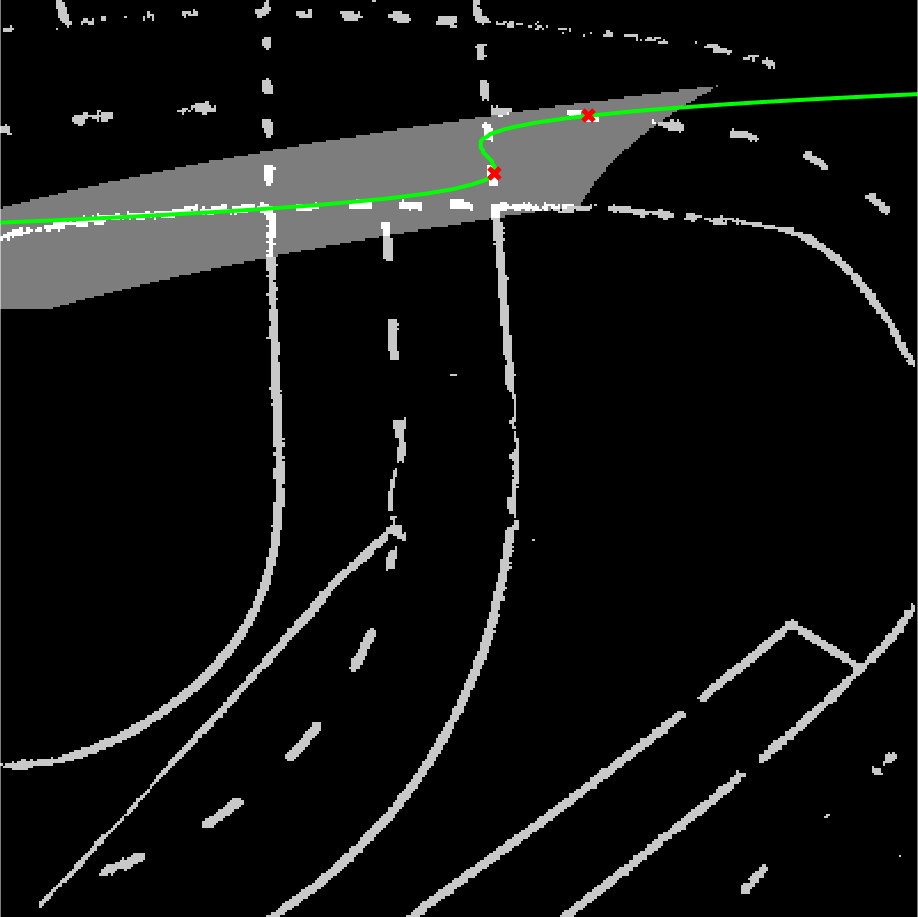
\includegraphics[width=0.31\textwidth]{evaluation_ransac_imgMaskLeft.png}}
	\quad
	\subfloat[][]{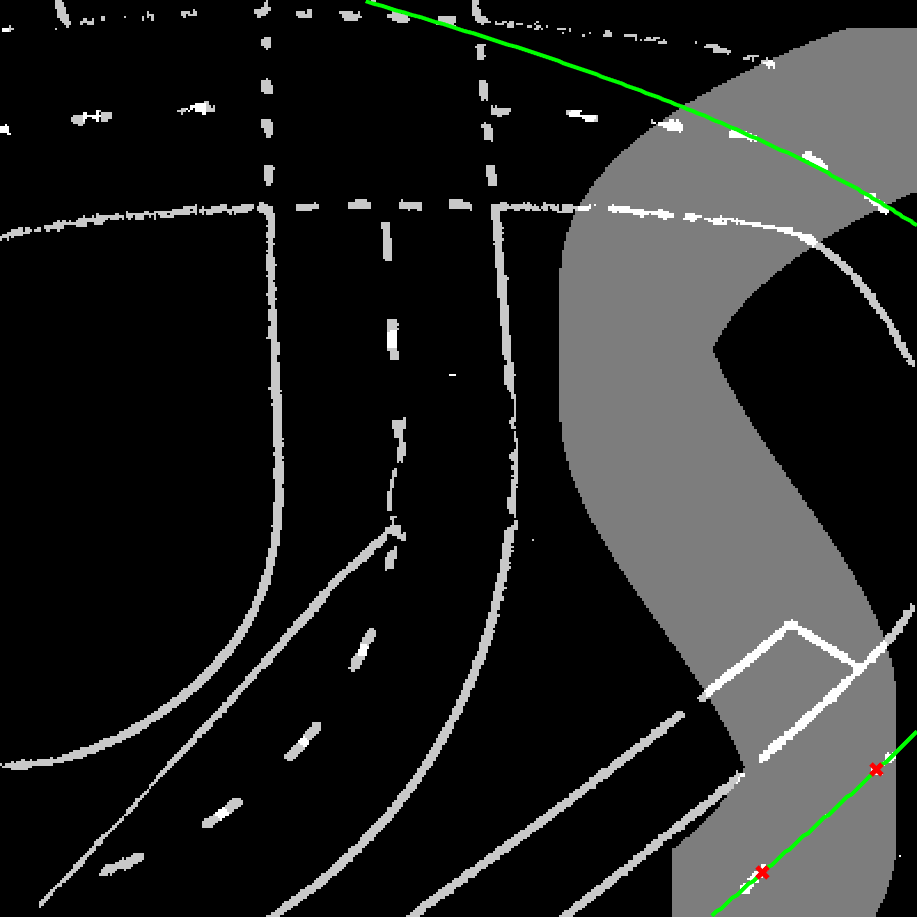
\includegraphics[width=0.31\textwidth]{evaluation_ransac_imgMaskMiddle.png}}
	\quad
	\subfloat[][]{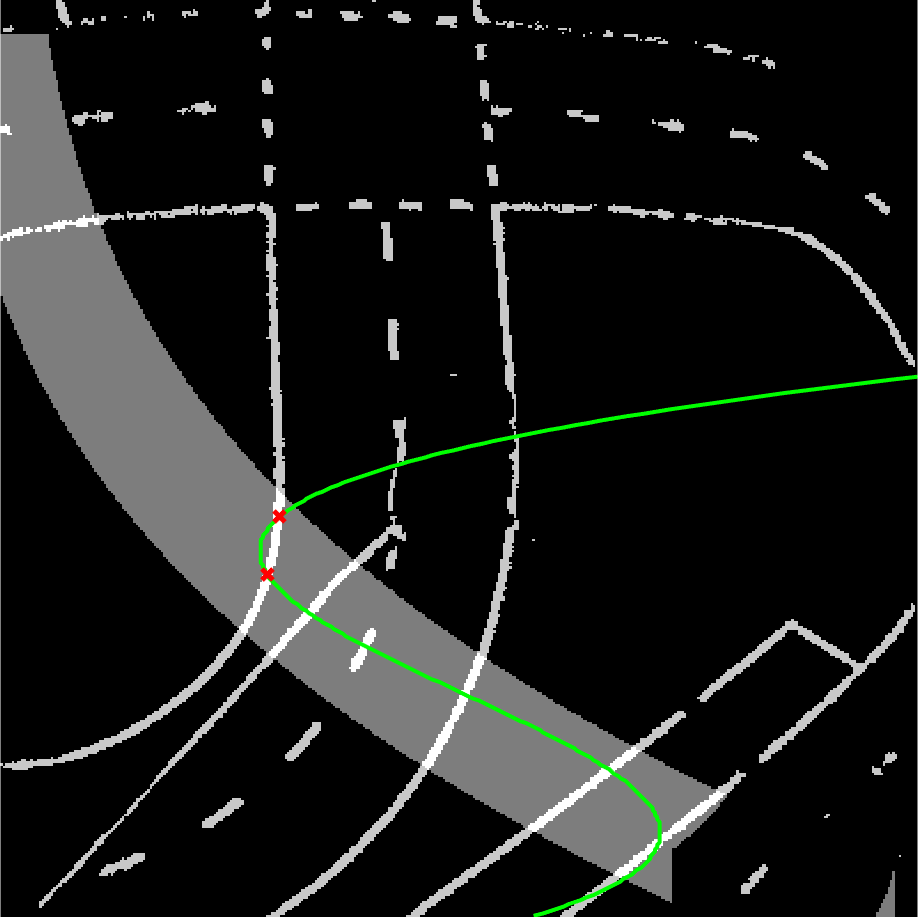
\includegraphics[width=0.31\textwidth]{evaluation_ransac_imgMaskRight.png}}
	\caption{Fehlerhaft erzeugte Masken der linken (a), mittleren (b) und rechten (c) Fahrbahnmarkierungen während eines Testlaufes}
	\label{fig:evaluation_ransac_ransac}
\end{figure} 

Das Polynom hat keine Chance, die Fahrbahnmarkierung richtig abzubilden, da sie nicht zu den Punkten des maskierten Bereichs gehört. Jene fehlerhaften \glspl{acr:roi} entstehen durch zuvor falsch erkannte, in die Weltkarte eingetragene Punkte. Abbildung~\ref{evaluation_ransac_weltkarte} zeigt das Ergebnis eines Testlaufs. Dieser wurde mit Hilfe einer Aufnahme (rosbag\footnote{Rosbag ist eine Reihe von Tools zum Aufnehmen und Wiedergeben von ROS-Topics (wiki.ros.org/rosbag)}) durchgeführt, welche während manueller Steuerung des Fahrzeugs entstanden ist. Im dargestellten Plot der Weltkarte ist die anfänglich zufriedenstellende Detektion der Fahrbahnmarkierungen zu erkennen, welche jedoch ab der ersten Kreuzung verloren geht.

% Bild/Plot der eingetragenen Punkte in der Weltkarte nach ein paar Sekunden
\begin{figure}[htbp] % [htb]
	\centering
	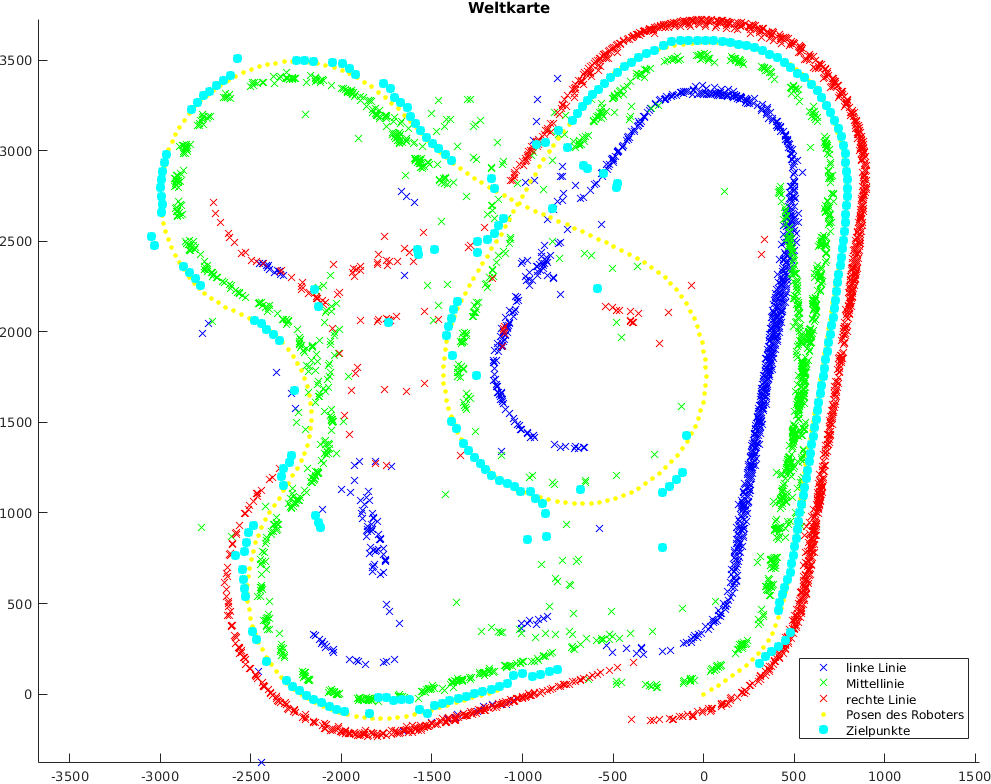
\includegraphics[width=1\textwidth]{evaluation_ransac_worldMap.png}
	\caption{Plot der Weltkarte nach einer Testrunde mittels manueller Steuerung}
	\label{evaluation_ransac_weltkarte}
\end{figure} 

Wenn in einem zuletzt untersuchten Bild keine Linienpunkte gefunden wurden, muss die Maske des übernächsten Bildes aus den zuletzt eingetragenen Punkten erstellt werden. Diese Punkte können ungünstigerweise weit von der jetzigen Position entfernt liegen, sodass stark extrapoliert werden muss. In dieser Entfernung zu den Stützstellen bildet das die Maske beschreibende Polynom den wirklichen Linienverlauf ungenügend ab und der \gls{acr:ransac} kann erneut keine richtigen Punkte finden. Somit ist die Voraussetzung gegeben, dass der Algorithmus im nächsten Foto erneut fehlschlägt, da falsche Punkte in der Karte zu noch stärkeren Abweichungen der Masken gegenüber der eigentlichen Markierung führen. Es entwickelt sich eine Kettenreaktion, die ein \glqq Sich-Wieder-Fangen\grqq{} des Algorithmus sehr unwahrscheinlich macht. 
Hinzu kommt, dass selbst bei ideal ausgewählten \glspl{acr:roi} die mathematische Beschreibung nicht jedem beliebigen Kurvenverlauf exakt folgen kann. 


\subsection{Lösungsmöglichkeiten}

Zugegebenerweise könnte der \gls{acr:ransac} mit Maskierungen zu einem stabilen Verfahren ausgebaut werden, wenn man eine Möglichkeit findet, die Bestimmung der \gls{acr:roi} zuverlässiger zu gestalten. Die Riverflow-Methode bot allerdings die vielversprechende Aussicht auf eine robuste Funktionsweise ohne aufwändige Anpassungen. 

Beispielsweise wäre es denkbar, die maximale Krümmung des kubischen Polynoms zu beschränken, um so ein Abdriften der Masken an Kreuzungen zu unterbinden. Da ein Polynom jedoch stets ins Unendliche läuft, wäre eine andere mathematische Beschreibung möglicherweise sinnvoller gewesen. Wenigstens die Masken könnten aus zusammengesetzten Kreisen oder Splines hervorgehen. Außerdem könnte man die Maskenbreite von der Entfernung bekannter Stützstellen abhängig machen, sodass in unbekannten Bereichen auf größerer Fläche gesucht werden kann. Zusätzlich wäre es möglich, die Masken durch die bekannte Fahrspurbreite voneinander abhängig zu machen, um ein Überlappen oder Vertauschen von linker und rechter Linie zu verhindern.

Falls im Rahmen weiterer Projekte der Riverflow-Algorithmus an seine Grenzen kommen sollte, ließe sich also unser erster Ansatz ebenfalls zum lauffähigen Programm erweitern. Unsere weitere Idee zur Verbesserung der Prädiktion einer Linie wird im nun folgenden Abschnitt zum Kalman ausgewertet.

